
\section{Membranas poliméricas de inclusión}\label{sec:pimint}\index{PIM}
Las membranas poliméricas de inclusión (PIM) son un tipo de membranas líquidas que incorporan extractantes en la red polimérica de un termoplástico no poroso. Las \ac{PIM}s tienen las ventajas que presentan las \ac{SLM}s (unificación de los pasos de extracción y recuperación, bajo consumo de extractantes y de disolventes), y superan el principal inconveniente de este tipo de membranas relacionado con su pobre estabilidad \citep{Nghiem2006}. A diferencia de las SLM, en una PIM los extractantes no se encuentran disueltos en un disolvente que está impregnado en los canales de una membrana porosa, sino que se encuentran absorbidos en la red polimérica por fuerzas capilares y de unión no covalente. Dado que los extractantes no se encuentran en contacto tan directo con las disoluciones acuosas, son más resistentes frente a la lixiviación hacia estas . 

Las \ac{PIM}s se encuentran en aplicaciones que van más allá de la separación selectiva de especies en disolución. Han sido utilizadas en distintas técnicas analíticas de cuantificación de especies (por métodos electroquímicos y espectrofotométricos), y de pretratamiento de muestras (preconcentración de especies y muestreo pasivo) \citep{ALMEIDA2017}. La separación selectiva de especies en disolución utilizando PIMs puede ser con fines extractivos, o para disminuir la peligrosidad de residuos mineros, industriales, y nucleares \citep{Kolev2019}.

El polímero base generalmente es de triacetato de celulosa (CTA) \acused{CTA} o de poli(cloruro de vinilo) (PVC) \acused{PVC}. El polímero se encarga de dar forma a la membrana y de proveerle resistencia mecánica. En la mayoría de los casos, se hace necesaria la adición de un plastificante que provee flexibilidad al polímero por medio de la disminución en las interacciones entre las cadenas poliméricas. Sin embargo, a veces la adición de un plastificante no es necesaria, pues las moléculas del extractante pueden cumplir también esa función. 

%\subsection{Extractantes}
%Los extractantes son la parte más importante en la \ac{PIM}. Las interacciones de estas moléculas con las especies en disolución dependen fuertemente de la naturaleza de la especie en cuestión por lo que éstos son los encargados de proveer la selectividad del proceso. Los extractantes 
    
%En la extracción de litio usando \ac{SLM}s o \ac{SSX} es común la combinación de un extractante ácido con un agente quelante. La combinación de extractantes de esta naturaleza presenta efectos sinérgicos que permiten la separación de litio que es muy difícil o imposible usando los mismos extractantes individualmente.

\subsection{Parámetros de desempeño}\label{sec:performanceparameters}
Una PIM puede caracterizarse por medio de la mayoría de las técnicas ampliamente esparcidas en la ciencia de materiales (e.g.\ microscopías electrónicas, análisis térmicos, métodos electroquímicos y espectrofotométricos). Cuando el propósito de la \ac{PIM} es transportar un elemento con el fin de lograr su recobro, es particularmente importante conocer la eficiencia con la que se lleva a cabo el proceso y el coeficiente de permeabilidad que está directamente relacionado con el flujo de la especie en cuestión a través de la membrana. Se espera que dicho recobro sea selectivo y la magnitud que permite juzgar la selectividad de un sistema es el factor de separación. Adicionalmente, desde un punto de vista práctico, una membrana robusta que pueda usarse varias veces es más viable que una membrana que solo funciona una vez. Los cambios en las propiedades de transporte de una membrana en el tiempo como consecuencia de alteraciones estructurales fisicoquímicas se conoce como su envejecimiento físico \citep{Koros}.

La eficiencia ($E$) en el proceso de transporte estudiado se relaciona con la concentración de ion litio que ha sido alcanzada en la fase de recuperación a un determinado tiempo $t$, respecto a la concentración inicialmente presente en la fase de alimentación. Usualmente se reporta en términos de porcentaje. Los datos del transporte pueden presentarse como fracción remanente en la disolución de alimentación ($\Phi_{ali}$), y fracción transportada a la disolución de recuperación ($\Phi_{rec}$), en función del tiempo. En este caso, la eficiencia se hace equivalente a la fracción transportada a la disolución de recuperación, en porcentaje.
\begin{equation}
    E(t)=\frac{[\ce{Li^+}]_{rec}(t)}{[\ce{Li^+}]_{ali}^0}\times100\% = \Phi_{rec}(t)\times100\%
\end{equation}

El coeficiente de permeabilidad ($P$) \index{Coeficiente de permeabilidad} se define como el flujo transportado a través de una membrana por unidad de fuerza motriz (gradiente de potencial químico en nuestro caso), por unidad de grosor de la membrana \citep{Koros}. En membranas líquidas se asume que las reacciones de formación/disociación de aductos en las interfases de la membrana son más rápidas que el proceso de difusión de la especie a través de la membrana. En ese caso, la ley de difusión de Fick en estado estacionario puede escribirse \citep{Ma2000}:
\begin{equation}\label{eq:fick}
    P=-\frac{d[\ce{Li^+}]_{ali}(t)}{dt}\times\frac{V}{a}\times\frac{1}{[\ce{Li^+}]_{ali}(t)}
\end{equation}
Donde $V$ es el volumen inicial de la disolución de alimentación y $a$ es el área expuesta de la membrana. La Ecuación diferencial \ref{eq:fick} puede resolverse por separación de términos e integración considerando que $[\ce{Li^+}]_{ali}(t=0)=[\ce{Li^+}]_{ali}^0$:
\begin{equation}
    \ln{\Bigg(\frac{[\ce{Li^+}]_{ali}(t)}{[\ce{Li^+}]_{ali}^0}\Bigg)}=\ln(\Phi_{ali}(t))=-\frac{P~a}{V}t
\end{equation}
En ese orden de ideas, el logaritmo natural de la fracción remanente de ion litio en la fase de alimentación debería ser una relación lineal negativa con el tiempo. A partir de la pendiente de dicha relación puede obtenerse el coeficiente de permeabilidad.

El factor de separación \index{Factor de separación} de ion litio frente a otro catión \ce{M^n+} ($Sf_{\ce{Li+}/\ce{M^n+}}$), se define como la relación de sus concentraciones en la disolución de recuperación respecto al valor inicial de esta relación en la fase de alimentación \citep{Chen2018}. Otras definiciones usan en el denominador la relación de las concentraciones en la disolución de alimentación al mismo tiempo $t$ \citep{Koros, sharma2016}. Estas definiciones son más apropiadas para sistemas de separación en sistemas continuos, y por lo tanto pueden conducir a conclusiones erróneas en sistemas como el trabajado en el presente proyecto. El factor de separación debe ser igual a uno al comienzo del experimento, indicando que no ha ocurrido separación de especies. Factores de separación más grandes implican mejor selectividad por la especie de interés. Un factor de separación menor a uno indica que la especie que no es de interés es transportada con preferencia a través de la membrana, es decir, que el sistema no es selectivo frente a dicha especie.
\begin{equation}
    Sf_{\ce{Li^+}/\ce{M^n+}}(t)=\frac{[\ce{Li^+}]_{rec}(t)/[\ce{M^n+}]_{rec}(t)}{[\ce{Li^+}]_{ali}^0/[\ce{M^n+}]_{ali}^0}
\end{equation}

Cuando el envejecimiento físico de la membrana es consecuencia de su utilización, éste puede determinarse de manera inversa como la estabilidad que presentan sus propiedades de transporte tras un número determinado de ciclos de uso.  La estabilidad de las PIMs es una de sus principales ventajas frente a otros sistemas de separación, y es quizás el parámetro clave que puede impulsar su aplicación en el mundo real. 

Finalmente, una manera práctica de evaluar el desempeño de un sistema frente a una sustancia es a través de su perfil de transporte, \index{Perfiles de transporte} que muestra gráficamente las fracciones o concentraciones de una o más especies, en las fases de alimentación y de recuperación, en función del tiempo. Los perfiles de transporte dan cuenta de la eficiencia de la extracción y la velocidad a la que ocurre el proceso. Si se incluye más de una especie en el perfil de transporte, esta herramienta también otorga información de la selectividad con la que se lleva a cabo el proceso.


\subsection{Mecanismo de extracción de ion litio con el sistema propuesto}
Para que una especie logre ser transportada a través de una \ac{PIM}, primero debe formarse el complejo de la especie de interés con los extractantes de la membrana en la interfase de la membrana con la disolución de alimentación, y dicho complejo debe difundir hasta la interfase de la membrana con la disolución de recuperación. Finalmente, el compuesto formado debe disociarse para liberar la especie en cuestión hacia la disolución de recuperación. Las reacciones que presenta el ion litio con los extractantes escogidos se tratan en este apartado.

Los procesos de transporte que involucran el transporte activo de sustancias facilitado por extractantes a través de PIMs, pueden utilizar como fuerza motriz el contratransporte de un catión, o de un anión, que se encuentra a altas concentraciones en la disolución de recuperación. También puede aprovecharse el cotransporte de un anión, o de un catión, que se encuentra a altas concentraciones en la disolución de alimentación \citep{Nghiem2006}. En el caso del transporte de ion litio, el proceso es impulsado por el contratransporte de iones hidronio que son tomados de la disolución de recuperación, y son liberados en la disolución de alimentación cada vez que se toma un ion litio de este medio.

Como se mencionó en la Sección \ref{sec:extr.disolv}, el número de coordinación del ion litio es de cuatro, y en medio acuoso la especie que predomina es el ion tetrahidratado \citep{Kinugasa1994}. Las aguas de hidratación del ion dificultan su paso a través de la membrana de \ac{CTA}, que es de naturaleza hidrofóbica \citep{Nghiem2006}. Las reacciones de formación y disociación de aductos que tienen lugar en las interfaces de la \ac{PIM} con las disoluciones de alimentación y de recuperación son prácticamente las mismas que se presentan en los sistemas análogos de extracción sinérgica con disolventes (SSX)\acused{SSX}, reportado por \citet{Pranolo2015}, y con \ac{SLM}, reportado por \citet{Ma2000}. Debe considerarse que a diferencia de las extracciones con disolventes, la cantidad de extractante disponible para reaccionar en una PIM puede ser limitada respecto a la cantidad de iones objetivo que deben ser transportados. Esto puede justificar que la selectividad de estos sistemas no necesariamente tiene que ser igual a la observada en los sistemas análogos de extracción por disolventes \citep{Nghiem2006}. 

Las reacciones que pueden estar ocurriendo en la interfase membrana/disolución-de-alimentación incluirían, en una primera etapa, la formación de un complejo del tautómero enólico del LIX-54-100 con el ion litio:

\begin{equation}\label{eq:li1}
    \scriptsize\schemestart
    \chemleft\{\chemfig{O=[:180]
        (-[:120](-[:60](=[:0]O)(-[:120,,,1]R_1)))
        (-[:-120]R_2)}\chemright.
     \arrow{<->} 
    \chemleft. \chemfig{O=[:180]
        (-[:120](=[:60]((-[:0]O-[:-30]H))(-[:120,,,1]R_1)))
        (-[:-120]R_2)}\chemright\}
    \,+\,
    \chemleft[\chemfig{\color{black}{Li^+}
    (-[:45,1.4,,,<-]OH_2)
    (-[:135,1.4,,,<-]H_2O)
    (-[:-45,1.4,,,<-]OH_2)
    (-[:-135,1.4,,,<-]H_2O)}\chemright]
    \arrow{<=>[-\ce{2H2O}][+\ce{2H2O}]}
    \chemleft[\chemfig{\color{black}{Li}
    (-[:45,1.2,,,<-]OH_2)
    (-[:135,1.2,,,]O
        -[:180](-[:120,,,1]R_1)(=[:-120]))
    (-[:-45,1.2,,,<-]OH_2)
    (-[:-135,1.2,,,<-]O
        =[:180](-[:120])(-[:-120]R_2))}\chemright] 
    \arrow{0}[,0]
    \,+\, \ce{H+}
    \schemestop
    %\bigskip
\end{equation}\\[0.01ex]
donde \ce{R_1} y \ce{R_2} pueden ser sustituyentes fenil y heptil.

En una segunda etapa, las dos moléculas de aguas de hidratación remanentes en la esfera de solvatación del ion litio son desplazadas de este lugar por el extractante solvatante Cyanex~923, con lo que el aducto resultante es altamente hidrofóbico y puede ser transportado a través de la membrana.

\begin{equation}\label{eq:li2}
    \scriptsize\schemestart
    \chemleft[ \chemfig{O(-[:45,,,,->])(=[:180]
        (-[:120](=[:60]((-[:0]O-[:-45,1.1]Li(-[:-45,1.2,,,<-]OH_2)(-[:45,1.2,,,<-]OH_2)))
        (-[:120,,,1]R_1)))
        (-[:-120]R_2))}\chemright]
    \,+\,
    \chemfig{P(=[:90]O)(-[:-45,1.3]R_3')(-[:-75,1.3]R_2')(-[:-115,1.3]R_1')}
    \arrow{<=>[-\ce{2H2O}][+\ce{2H2O}]}
    \chemleft[ \chemfig{O(-[:45,,,,->])(=[:180]
        (-[:120](=[:60]((-[:0]O-[:-45,1.1]Li(-[:30,1.3,,,<-]O(=[:-90, 1.3]P
            (-[:-45,1.3]R_3')(-[:-75,1.3]R_2')(-[:-115,1.3]R_1')))-[:-30,1,,,<-]))
        (-[:120,,,1]R_1)))
        (-[:-120]R_2))}\chemright]
    \schemestop
    \bigskip
\end{equation}
donde \ce{R_1}', \ce{R_2}', y \ce{R_3}' son cadenas alquílicas con seis u ocho átomos de carbono.

Las Reacciones \ref{eq:li1} y \ref{eq:li2} ocurren en la dirección planteada en la interfase con la disolución de alimentación, y en la dirección contraria en la interfase con la disolución de recuperación. El resultado neto es el transporte de ion litio hacia la disolución de recuperación con el  consecuente transporte de iones hidronio hacia la disolución de alimentación.



%\section{Técnicas de cuantificación empleadas}
%\subsection{Espectrometría de Absorción Atómica por Llama}
%\subsection{Espectrometría de Emisión Atómica por Llama}
%\subsection{Curva de calibración por patron externo}
%\subsection{Curva de calibración multivariada}
%\subsection{Adición estándar de un solo punto}

\section{Diseño de experimentos y optimización}\label{sec:DoE}\index{Diseño de experimentos}
En las ciencias exactas es común el estudio de sistemas en los que se busca relacionar un fenómeno con sus posibles causas. En algunos casos dicho conocimiento permite controlar o predecir propiedades de interés del sistema (i.e.\ variables respuesta), tomando como base las condiciones que se cree que gobiernan al fenómeno en cuestión (i.e.\ variables explicatorias). Las variables explicatorias pueden estar compuestas por factores difíciles o imposibles de controlar (e.g.\ condiciones metereo\-lógicas), o bien, por parámetros que pueden ser ajustados al criterio del experimentador.

Tradicionalmente, esta clase de estudios se han hecho por un enfoque de una variable a la vez en la que se mantienen constantes la mayor cantidad posible de factores, a excepción de una variable que es modificada para buscar su relación con la variable respuesta de interés. Cuando se ha establecido esa relación, se escoge un valor conveniente que es fijado para la variable explicatoria recién estudiada, y el proceso se repite consecutivamente con otra variable hasta que todas han sido estudiadas. Esta metodología ha permitido aportes muy significativos en distintos campos y aún hoy por hoy es la opción predilecta por muchas personas que trabajan en campos muy importantes de la ciencia. Sin embargo, el enfoque de una variable a la vez presenta algunas limitaciones como el requerir un gran número de corridas experimentales y no evaluar las posibles interacciones entre variables explicatorias. Una consecuencia común de estas falencias metodológicas recae en que las condiciones encontradas como {óptimas} dependen en gran medida del orden en que son estudiadas las variables. En muchos casos esto implica que no se determine el punto óptimo real de un sistema.

Los diseños de experimentos y los algoritmos de optimización comprenden un conjunto de herramientas estadísticas y matemáticas que facilitan la planeación eficiente y el análisis objetivo de conjuntos experimentales. El propósito de estas herramientas es obtener la mayor cantidad posible de información de un sistema, o de llegar a su configuración más apropiada para un fin determinado (i.e.\ el punto óptimo), en un reducido número de experimentos \citep{Box2005}. 

Los conceptos de esta rama de la ciencia pueden ser aplicados para encontrar las mejores condiciones para el transporte de ion litio usando PIMs, considerando por ejemplo, el efecto de la formulación de la membrana en la eficiencia y la selectividad de los sistemas propuestos. En el desarro\-llo de esta tesis se han utilizado en particular los diseños experimentales fraccionados de dos niveles y el algoritmo de optimización simplex modificado. Las características más importantes de estos conceptos se exponen en las siguientes subsecciones.

\subsection{Diseño factorial fraccionado}\label{sec:FrF2introd}\index{Diseño de experimentos!factorial fraccionado}
En los diseños experimentales factoriales se estudia un número de variables $k$ en un número de niveles $n$ considerando todas las combinaciones posibles. El número de experimentos que deben realizarse es de $n^k$. Este valor crece considerablemente cuando se incluyen más niveles o variables. Aunque puede obtenerse información muy detallada del sistema, llevar a cabo un número tan grande de experimentos no es conveniente en la mayoría de los casos desde un punto de vista práctico. En el caso más simple y más famoso, los diseños experimentales factoriales son reducidos a solo $n=2$ niveles, pero el número de experimentos que deben realizarse en el estudio de $k$ variables sigue creciendo de manera exponencial a medida que se desea considerar más factores. La realización de $2^k$ experimentos permite, en principio, conocer el efecto de todas las variables en el sistema, incluyendo todas las interacciones que pueden presentar estas entre sí.

Con regularidad, la evaluación de las interacciones de alto grado (i.e.\ entre muchas variables) puede resultar de poca relevancia práctica, dado que la mayoría de las veces el efecto de dicha interacción no puede distinguirse del mero error aleatorio del proceso. En otras palabras, no es estadísticamente significativo. Esta consideración permite la realización de un número de experimentos mucho menor a expensas de la imposibilidad de determinar interacciones que se consideran poco importantes. Este es el principio de los diseños factoriales fraccionados en los que solo una fracción de la matriz de diseño es evaluada. La fracción debe escogerse cuidadosamente, de manera tal que la porción que se descarta no impida la evaluación de los efectos que se desea evaluar. Convenientemente, los algoritmos que permiten la elección de la {mejor fracción} se encuentran implementados en muchos programas y paquetes estadísticos \citep{FrF2}, por lo que esta decisión no es un problema para el experimentador en estos tiempos modernos.

Por ejemplo, en un diseño experimental factorial en el que se desea estudiar siete variables a dos niveles, el número de experimentos que debe correrse es de $2^7=128$. Sí se acepta que la interacción entre más de cuatro variables no es relevante, el mismo número de variables puede ser evaluado en $2^{7-1}=64$ experimentos. La reducción en el tiempo que debe invertirse es drástica. De manera análoga, si se ignoran las interacciones entre tres y en el caso más extremo, las interacciones entre parejas de variables, el número de experimentos a realizarse decrece a $2^{7-3}=16$ y $2^{7-4}=8$, respectivamente. 

Debe considerarse que los efectos de las interacciones entre variables no {desaparecen} cuando se decide que no es importante su determinación. Estos efectos se solapan con aquellos de inter\-accio\-nes de menor grado y con efectos de variables individuales. Cuando esto ocurre se dice que los efectos están {confundidos}. El hecho de que algunos efectos de variables puedan estar confundidos con interacciones que resulten relevantes es la principal desventaja de esta clase de diseños. Sin embargo, es importante recalcar que no todo lo que es significativo desde un punto de vista estadístico resulta importante desde un punto de vista práctico y la pericia del investigador siempre es un papel importante que va de la mano de los procedimientos estadísticos que tengan lugar. En todo caso, los métodos estadísticos no pueden considerarse totalmente confiables y su poder solo aumenta con el número de datos que pueden analizarse. Obtener más datos implica realizar más experimentos por lo que el experimentador debe considerar la cantidad de tiempo y recursos que está dispuesto a invertir para obtener respuestas a sus preguntas.

El propósito principal de los diseños experimentales factoriales fraccionados es el de otorgar un panorama general del efecto de las variables consideradas con el fin de determinar las que resultan importantes en el fenómeno que se estudia (i.e.\ cribado de variables), o de establecer una ruta que debe tomarse para efectuar experimentos posteriores. 

Las variables estadísticamente significativas pueden encontrarse por medio de un análisis de varianza sobre los efectos de las variables, pero en muchos casos el número de grados de libertad de los residuales es de cero debido al pequeño número de experimentos que se evalúan. El diagrama de efectos estandarizados de Pareto permite determinar de manera sencilla que variables son importantes, pero se requiere un estimador independiente de la variabilidad del método y dicho estimador no siempre está disponible. 

\citet{Daniel1959} propuso el uso de diagramas de probabilidad normal de los efectos estandarizados y probabilidad normal de los efectos estandarizados absolutos para determinar las variables estadísticamente significativas de una manera independiente del estimador de la variabilidad del método. Los {diagramas de Daniel} presentan una herramienta valiosa para el análisis de diseños experimentales factoriales fraccionados \citep{Box2005}. La principal desventaja que presenta la metodología propuesta es que otorga resultados más concisos en diseños de experimentos grandes (i.e.\ varios puntos experimentales) y por lo general no se obtiene un panorama claro en diseños experimentales fraccionados de solo ocho experimentos \citep{FrF2}. Adicionalmente, el uso de diagramas de Daniel supone que la mayoría de las variables no tienen un efecto importante en la respuesta. Si el supuesto de {escasez de efectos} no se cumple (i.e.\ si muchas va\-ria\-bles tienen efectos estadísticamente significativos), los diagramas de Daniel pueden no otorgar una visión clara del estudio realizado. \index{Diagramas de Daniel} 

\citet{Lenth1989} propuso un método numérico para determinar las variables estadísticamente significativas en diseños factoriales fraccionados. El método propuesto también es independiente del estimador de la variabilidad del proceso bajo estudio, pero a diferencia de los diagramas de Daniel, su interpretación no es susceptible a subjetividades dado que pueden obtenerse valores de probabilidad que pueden compararse con la significancia escogida. La significancia que se escoge en la determinación de variables importantes es por lo general algo {generosa} (0.10. en lugar del valor más tradicional de 0.05), dado que es menos perjudicial considerar una variable adicional que resulta ser poco importante (error tipo I), respecto a no considerar una variable cuyo efecto es estadísticamente significativo (error tipo II) \citep{FrF2}.

Cuando se han eliminado las variables con efectos poco importantes el modelo se dice que se ha reducido. Los resultados del {modelo reducido} pueden analizarse por medio de un método lineal que puede indicar la dirección en la que la respuesta del sistema es mejor.


\subsubsection{Propuesta de estimación de variables importantes}\label{app:ParedesMethod}
Una posibilidad adicional para determinar que variables son importantes se plantea en el presente trabajo e involucra el estudio de los resultados del diseño a través de regresiones lineales, contemplando inicialmente modelos lo más simples posibles (una sola variable explicatoria a la vez). Estos modelos son sometidos a un análisis de varianza de los parámetros de regresión involucrados para determinar que variables son estadísticamente significativas. El proceso debe iterarse con modelos que son complementados paulatinamente con más variables, añadiendo una a la vez y probando todas las combinaciones posibles.

Cuando se consideran menos variables explicatorias de las que se utilizaron para elaborar la matriz de diseño, los residuales de la regresión quedan con suficientes grados de libertad para un análisis de varianza sobre los parámetros de la regresión (i.e.\ las variables consideradas). Las variables que resulten estadísticamente significativas en alguna de las corridas deben ser consideradas para su posterior estudio de la misma manera como se hace con las que se identifican como importantes utilizando los otros métodos.

La propuesta que se hace también es independiente del estimador de la variabilidad propia del sistema, y si bien su procedimiento puede parecer tedioso, su implementación en algún programa estadístico (como el aclamado \R), puede lograr su automatización de manera que la obtención de resultados no represente una vasta inversión de tiempo.


\subsection{Algoritmo símplex modificado}\index{Diseño de experimentos!algoritmo símplex}
El algoritmo de optimización símplex, propuesto en un comienzo por \citet{Spendley1962} y posteriormente modificado por \citet{Nelder1965}, plantea la abstracción del fenómeno bajo estudio como un espacio $n$-dimensional en el que cada dimensión está conformada por una variable. Un determinado punto en dicho espacio $n$-dimensional tiene $n$ coordenadas que en el mundo real representan los valores que toman las $n$ variables explicatorias que se consideran. El algoritmo hace uso de un objeto geométrico (símplex) que está definido para espacios de cualquier dimensionalidad y que se caracteriza por ser el politopo\footnote{Generalización $n$-dimensional de un objeto con \textit{caras} planas. En dos dimensiones los politopos de denominan polígonos y en tres dimensiones, poliedros.} más simple posible en dicho espacio. En espacios bidimensionales el politopo más simple (símplex) es un triángulo, y en espacios tridimensionales, un tetraedro. 

Los simplexes se caracterizan por tener un número de vértices igual a la dimensionalidad del espacio más uno. Cada vértice del simplex representa un experimento que se lleva a cabo bajo las condiciones que dictaminan sus {coordenadas} para cada variable. Las respuestas de los experimentos definidos por cada vértice caen en la superficie de respuesta del fenómeno bajo estudio y en principio, algunos valores caerán más cerca de un máximo local (o mínimo local), que representa el punto óptimo del proceso que se desea optimizar. La estrategia del algoritmo supone que es posible acercarse al punto óptimo por medio de movimientos que se alejan del punto más malo. 

Desde un punto de vista práctico, se propone un conjunto de experimentos que definen los vértices del símplex inicial. Por las características del simplex, en el estudio de $k$ variables, tienen que hacerse $k+1$ experimentos diferentes. Las coordenadas de los vértices del símplex inicial deben escogerse de manera tal que el objeto tenga un hipervolumen\footnote{Porción de espacio ocupado por un objeto en un espacio $n$-dimensional. Es la generalización del volumen para politopos de espacios con más de tres dimensiones.} no nulo. Cuando se han realizado los experimentos y se ha obtenido una respuesta para cada uno de ellos, se descarta uno de los vértices en función de uno nuevo que debe evaluarse. Este proceso debe repetirse iterativamente hasta que se alcanza una respuesta satisfactoria o hasta que el algoritmo determina que se ha llegado a un máximo local.

El vértice que debe ser descartado y el nuevo que debe ser evaluado se escoge con base en reglas sencillas que involucran operaciones aritméticas básicas que se traducen en {movimientos del simplex}. El algoritmo original de 1962 contempla únicamente la {reflexión}, cuyo efecto es la generación de un nuevo símplex que resulta de la imagen especular del símplex original al descartar el punto más indeseable. Las modificaciones de 1965 incluyeron tres posibles movimientos adicionales: {expansión}, {contracción del lado del vértice descartado} y {contracción del lado del vértice reflejado}. Los posibles movimientos de un símplex en un espacio bidimensional se ilustran en la Figura \ref{fig:Simplexmov}.

\begin{figure}[htbp]
    \centering
    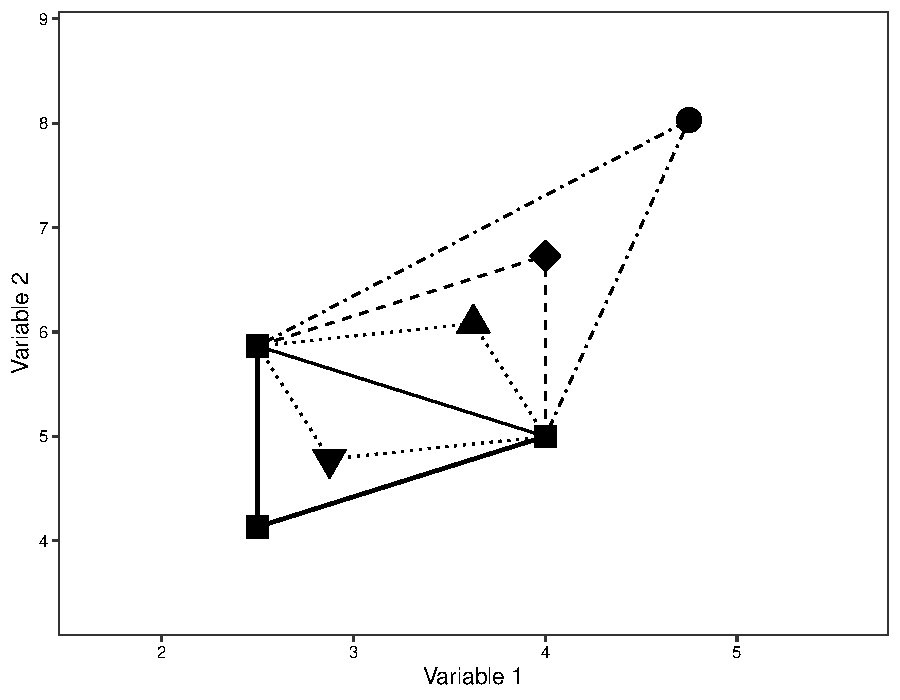
\includegraphics[width=0.6\textwidth]{chap2/images/simplexmov.pdf}
    \caption[Posibles movimientos de un símplex en un espacio bidimensional.]{Posibles movimientos de un símplex en un espacio bidimensional. Símplex original (\protect\squareblck), reflexión (\protect\squarerttdblck), expansión (\protect\circleblck), contracción del lado de la reflexión (\protect\triangleupblck) y contracción del lado del peor vértice (\protect\triangledownblck).}
    \label{fig:Simplexmov}
\end{figure}

Una de las ventajas más remarcables del algoritmo de optimización símplex es que el número de experimentos a realizar no crece de manera abrupta cuando se decide incluir más variables en el estudio. Por ejemplo, si en un diseño factorial a dos niveles se decide evaluar cuatro variables en lugar de tres, el número de experimentos de la matriz de diseño cambia de 8 a 16. Para la evaluación del simplex inicial, el número de experimentos cambia de cuatro a cinco. Esto hace menos importante el cribado de variables importantes que se recomienda antes del desarrollo de un diseño experimental más complejo.% (e.g.\ Matriz de Doehlert \citep{FERREIRA2004}).

El detalle de las reglas que gobiernan los algoritmos de optimización símplex y símplex modificado se describen con claridad en los capítulos tercero y cuarto del libro de \citet{simplexbook}. Ambos algoritmos han sido implementados en un paquete del lenguaje de programación \verb|R|. El paquete \verb|labsimplex| se encuentra disponible en de CRAN, y provee de herramientas para diseñar el símplex inicial, generar los vértices nuevos, visualizar gráficamente los movimientos del símplex y la evolución en la respuesta, entre otras cosas \citep{labsimplex}.